
%% bare_conf.tex
%% V1.4
%% 2012/12/27
%% by Michael Shell
%% See:
%% http://www.michaelshell.org/
%% for current contact information.
%%
%% This is a skeleton file demonstrating the use of IEEEtran.cls
%% (requires IEEEtran.cls version 1.8 or later) with an IEEE conference paper.
%%
%% Support sites:
%% http://www.michaelshell.org/tex/ieeetran/
%% http://www.ctan.org/tex-archive/macros/latex/contrib/IEEEtran/
%% and
%% http://www.ieee.org/

%%*************************************************************************
%% Legal Notice:
%% This code is offered as-is without any warranty either expressed or
%% implied; without even the implied warranty of MERCHANTABILITY or
%% FITNESS FOR A PARTICULAR PURPOSE! 
%% User assumes all risk.
%% In no event shall IEEE or any contributor to this code be liable for
%% any damages or losses, including, but not limited to, incidental,
%% consequential, or any other damages, resulting from the use or misuse
%% of any information contained here.
%%
%% All comments are the opinions of their respective authors and are not
%% necessarily endorsed by the IEEE.
%%
%% This work is distributed under the LaTeX Project Public License (LPPL)
%% ( http://www.latex-project.org/ ) version 1.3, and may be freely used,
%% distributed and modified. A copy of the LPPL, version 1.3, is included
%% in the base LaTeX documentation of all distributions of LaTeX released
%% 2003/12/01 or later.
%% Retain all contribution notices and credits.
%% ** Modified files should be clearly indicated as such, including  **
%% ** renaming them and changing author support contact information. **
%%
%% File list of work: IEEEtran.cls, IEEEtran_HOWTO.pdf, bare_adv.tex,
%%                    bare_conf.tex, bare_jrnl.tex, bare_jrnl_compsoc.tex,
%%                    bare_jrnl_transmag.tex
%%*************************************************************************

% *** Authors should verify (and, if needed, correct) their LaTeX system  ***
% *** with the testflow diagnostic prior to trusting their LaTeX platform ***
% *** with production work. IEEE's font choices can trigger bugs that do  ***
% *** not appear when using other class files.                            ***
% The testflow support page is at:
% http://www.michaelshell.org/tex/testflow/



% Note that the a4paper option is mainly intended so that authors in
% countries using A4 can easily print to A4 and see how their papers will
% look in print - the typesetting of the document will not typically be
% affected with changes in paper size (but the bottom and side margins will).
% Use the testflow package mentioned above to verify correct handling of
% both paper sizes by the user's LaTeX system.
%
% Also note that the "draftcls" or "draftclsnofoot", not "draft", option
% should be used if it is desired that the figures are to be displayed in
% draft mode.
%
\documentclass[conference]{IEEEtran}
% Add the compsoc option for Computer Society conferences.
%
% If IEEEtran.cls has not been installed into the LaTeX system files,
% manually specify the path to it like:
% \documentclass[conference]{../sty/IEEEtran}





% Some very useful LaTeX packages include:
% (uncomment the ones you want to load)


% *** MISC UTILITY PACKAGES ***
%
%\usepackage{ifpdf}
% Heiko Oberdiek's ifpdf.sty is very useful if you need conditional
% compilation based on whether the output is pdf or dvi.
% usage:
% \ifpdf
%   % pdf code
% \else
%   % dvi code
% \fi
% The latest version of ifpdf.sty can be obtained from:
% http://www.ctan.org/tex-archive/macros/latex/contrib/oberdiek/
% Also, note that IEEEtran.cls V1.7 and later provides a builtin
% \ifCLASSINFOpdf conditional that works the same way.
% When switching from latex to pdflatex and vice-versa, the compiler may
% have to be run twice to clear warning/error messages.






% *** CITATION PACKAGES ***
%
%\usepackage{cite}
% cite.sty was written by Donald Arseneau
% V1.6 and later of IEEEtran pre-defines the format of the cite.sty package
% \cite{} output to follow that of IEEE. Loading the cite package will
% result in citation numbers being automatically sorted and properly
% "compressed/ranged". e.g., [1], [9], [2], [7], [5], [6] without using
% cite.sty will become [1], [2], [5]--[7], [9] using cite.sty. cite.sty's
% \cite will automatically add leading space, if needed. Use cite.sty's
% noadjust option (cite.sty V3.8 and later) if you want to turn this off
% such as if a citation ever needs to be enclosed in parenthesis.
% cite.sty is already installed on most LaTeX systems. Be sure and use
% version 4.0 (2003-05-27) and later if using hyperref.sty. cite.sty does
% not currently provide for hyperlinked citations.
% The latest version can be obtained at:
% http://www.ctan.org/tex-archive/macros/latex/contrib/cite/
% The documentation is contained in the cite.sty file itself.






% *** GRAPHICS RELATED PACKAGES ***
%
\ifCLASSINFOpdf
  \usepackage[pdftex]{graphicx}
  % declare the path(s) where your graphic files are
  \graphicspath{{../pdf/}{../jpeg/}{./img}}
  % and their extensions so you won't have to specify these with
  % every instance of \includegraphics
  \DeclareGraphicsExtensions{.pdf,.jpeg,.png,.pdf}
\else
  % or other class option (dvipsone, dvipdf, if not using dvips). graphicx
  % will default to the driver specified in the system graphics.cfg if no
  % driver is specified.
  % \usepackage[dvips]{graphicx}
  % declare the path(s) where your graphic files are
  % \graphicspath{{../eps/}}
  % and their extensions so you won't have to specify these with
  % every instance of \includegraphics
  % \DeclareGraphicsExtensions{.eps}
\fi
% graphicx was written by David Carlisle and Sebastian Rahtz. It is
% required if you want graphics, photos, etc. graphicx.sty is already
% installed on most LaTeX systems. The latest version and documentation
% can be obtained at: 
% http://www.ctan.org/tex-archive/macros/latex/required/graphics/
% Another good source of documentation is "Using Imported Graphics in
% LaTeX2e" by Keith Reckdahl which can be found at:
% http://www.ctan.org/tex-archive/info/epslatex/
%
% latex, and pdflatex in dvi mode, support graphics in encapsulated
% postscript (.eps) format. pdflatex in pdf mode supports graphics
% in .pdf, .jpeg, .png and .mps (metapost) formats. Users should ensure
% that all non-photo figures use a vector format (.eps, .pdf, .mps) and
% not a bitmapped formats (.jpeg, .png). IEEE frowns on bitmapped formats
% which can result in "jaggedy"/blurry rendering of lines and letters as
% well as large increases in file sizes.
%
% You can find documentation about the pdfTeX application at:
% http://www.tug.org/applications/pdftex





% *** MATH PACKAGES ***
%
%\usepackage[cmex10]{amsmath}
% A popular package from the American Mathematical Society that provides
% many useful and powerful commands for dealing with mathematics. If using
% it, be sure to load this package with the cmex10 option to ensure that
% only type 1 fonts will utilized at all point sizes. Without this option,
% it is possible that some math symbols, particularly those within
% footnotes, will be rendered in bitmap form which will result in a
% document that can not be IEEE Xplore compliant!
%
% Also, note that the amsmath package sets \interdisplaylinepenalty to 10000
% thus preventing page breaks from occurring within multiline equations. Use:
%\interdisplaylinepenalty=2500
% after loading amsmath to restore such page breaks as IEEEtran.cls normally
% does. amsmath.sty is already installed on most LaTeX systems. The latest
% version and documentation can be obtained at:
% http://www.ctan.org/tex-archive/macros/latex/required/amslatex/math/


% *** SPECIALIZED LIST PACKAGES ***
%
%\usepackage{algorithmic}
% algorithmic.sty was written by Peter Williams and Rogerio Brito.
% This package provides an algorithmic environment fo describing algorithms.
% You can use the algorithmic environment in-text or within a figure
% environment to provide for a floating algorithm. Do NOT use the algorithm
% floating environment provided by algorithm.sty (by the same authors) or
% algorithm2e.sty (by Christophe Fiorio) as IEEE does not use dedicated
% algorithm float types and packages that provide these will not provide
% correct IEEE style captions. The latest version and documentation of
% algorithmic.sty can be obtained at:
% http://www.ctan.org/tex-archive/macros/latex/contrib/algorithms/
% There is also a support site at:
% http://algorithms.berlios.de/index.html
% Also of interest may be the (relatively newer and more customizable)
% algorithmicx.sty package by Szasz Janos:
% http://www.ctan.org/tex-archive/macros/latex/contrib/algorithmicx/
 \usepackage{algorithmicx}
 \usepackage[ruled]{algorithm}
 \usepackage{algpseudocode}





% *** ALIGNMENT PACKAGES ***
%
%\usepackage{array}
% Frank Mittelbach's and David Carlisle's array.sty patches and improves
% the standard LaTeX2e array and tabular environments to provide better
% appearance and additional user controls. As the default LaTeX2e table
% generation code is lacking to the point of almost being broken with
% respect to the quality of the end results, all users are strongly
% advised to use an enhanced (at the very least that provided by array.sty)
% set of table tools. array.sty is already installed on most systems. The
% latest version and documentation can be obtained at:
% http://www.ctan.org/tex-archive/macros/latex/required/tools/


% IEEEtran contains the IEEEeqnarray family of commands that can be used to
% generate multiline equations as well as matrices, tables, etc., of high
% quality.




% *** SUBFIGURE PACKAGES ***
\ifCLASSOPTIONcompsoc
  \usepackage[caption=false,font=normalsize,labelfont=sf,textfont=sf]{subfig}
\else
  \usepackage[caption=false,font=footnotesize]{subfig}
\fi
% subfig.sty, written by Steven Douglas Cochran, is the modern replacement
% for subfigure.sty, the latter of which is no longer maintained and is
% incompatible with some LaTeX packages including fixltx2e. However,
% subfig.sty requires and automatically loads Axel Sommerfeldt's caption.sty
% which will override IEEEtran.cls' handling of captions and this will result
% in non-IEEE style figure/table captions. To prevent this problem, be sure
% and invoke subfig.sty's "caption=false" package option (available since
% subfig.sty version 1.3, 2005/06/28) as this is will preserve IEEEtran.cls
% handling of captions.
% Note that the Computer Society format requires a larger sans serif font
% than the serif footnote size font used in traditional IEEE formatting
% and thus the need to invoke different subfig.sty package options depending
% on whether compsoc mode has been enabled.
%
% The latest version and documentation of subfig.sty can be obtained at:
% http://www.ctan.org/tex-archive/macros/latex/contrib/subfig/




% *** FLOAT PACKAGES ***
%
%\usepackage{fixltx2e}
% fixltx2e, the successor to the earlier fix2col.sty, was written by
% Frank Mittelbach and David Carlisle. This package corrects a few problems
% in the LaTeX2e kernel, the most notable of which is that in current
% LaTeX2e releases, the ordering of single and double column floats is not
% guaranteed to be preserved. Thus, an unpatched LaTeX2e can allow a
% single column figure to be placed prior to an earlier double column
% figure. The latest version and documentation can be found at:
% http://www.ctan.org/tex-archive/macros/latex/base/


%\usepackage{stfloats}
% stfloats.sty was written by Sigitas Tolusis. This package gives LaTeX2e
% the ability to do double column floats at the bottom of the page as well
% as the top. (e.g., "\begin{figure*}[!b]" is not normally possible in
% LaTeX2e). It also provides a command:
%\fnbelowfloat
% to enable the placement of footnotes below bottom floats (the standard
% LaTeX2e kernel puts them above bottom floats). This is an invasive package
% which rewrites many portions of the LaTeX2e float routines. It may not work
% with other packages that modify the LaTeX2e float routines. The latest
% version and documentation can be obtained at:
% http://www.ctan.org/tex-archive/macros/latex/contrib/sttools/
% Do not use the stfloats baselinefloat ability as IEEE does not allow
% \baselineskip to stretch. Authors submitting work to the IEEE should note
% that IEEE rarely uses double column equations and that authors should try
% to avoid such use. Do not be tempted to use the cuted.sty or midfloat.sty
% packages (also by Sigitas Tolusis) as IEEE does not format its papers in
% such ways.
% Do not attempt to use stfloats with fixltx2e as they are incompatible.
% Instead, use Morten Hogholm'a dblfloatfix which combines the features
% of both fixltx2e and stfloats:
%
% \usepackage{dblfloatfix}
% The latest version can be found at:
% http://www.ctan.org/tex-archive/macros/latex/contrib/dblfloatfix/




% *** PDF, URL AND HYPERLINK PACKAGES ***
%
%\usepackage{url}
% url.sty was written by Donald Arseneau. It provides better support for
% handling and breaking URLs. url.sty is already installed on most LaTeX
% systems. The latest version and documentation can be obtained at:
% http://www.ctan.org/tex-archive/macros/latex/contrib/url/
% Basically, \url{my_url_here}.




% *** Do not adjust lengths that control margins, column widths, etc. ***
% *** Do not use packages that alter fonts (such as pslatex).         ***
% There should be no need to do such things with IEEEtran.cls V1.6 and later.
% (Unless specifically asked to do so by the journal or conference you plan
% to submit to, of course. )


% correct bad hyphenation here
\hyphenation{op-tical net-works semi-conduc-tor}

% Miscallaneous packages
\usepackage{color}


\begin{document}
%
% paper title
% can use linebreaks \\ within to get better formatting as desired
% Do not put math or special symbols in the title.
\title{Implementation of Boruvka Algorithm for Minimum Spanning Tree Search on Charm++}


% author names and affiliations
% use a multiple column layout for up to three different
% affiliations
\author{
\IEEEauthorblockN{Alexander Frolov}
\IEEEauthorblockA{Science and Research \\ Centre of Computer Technology \\
NICEVT\\
Varshavskoe sh. 125, Moscow, Russia\\
Email: frolov@nicevt.ru}
\and
\IEEEauthorblockN{Alexander Semenov}
\IEEEauthorblockA{Science and Research \\ Centre of Computer Technology \\
NICEVT\\
Varshavskoe sh. 125, Moscow, Russia\\
Email: semenov@nicevt.ru}
%\IEEEauthorblockN{Mikhail Gilmendinov}
%\IEEEauthorblockA{Science and Research \\ Centre of Computer Technology \\
%NICEVT\\
%Varshavskoe sh. 125, Moscow, Russia\\
%Email: gilmendinov@nicevt.ru}
}

% conference papers do not typically use \thanks and this command
% is locked out in conference mode. If really needed, such as for
% the acknowledgment of grants, issue a \IEEEoverridecommandlockouts
% after \documentclass

% for over three affiliations, or if they all won't fit within the width
% of the page, use this alternative format:
% 
%\author{\IEEEauthorblockN{Michael Shell\IEEEauthorrefmark{1},
%Homer Simpson\IEEEauthorrefmark{2},
%James Kirk\IEEEauthorrefmark{3}, 
%Montgomery Scott\IEEEauthorrefmark{3} and
%Eldon Tyrell\IEEEauthorrefmark{4}}
%\IEEEauthorblockA{\IEEEauthorrefmark{1}School of Electrical and Computer Engineering\\
%Georgia Institute of Technology,
%Atlanta, Georgia 30332--0250\\ Email: see http://www.michaelshell.org/contact.html}
%\IEEEauthorblockA{\IEEEauthorrefmark{2}Twentieth Century Fox, Springfield, USA\\
%Email: homer@thesimpsons.com}
%\IEEEauthorblockA{\IEEEauthorrefmark{3}Starfleet Academy, San Francisco, California 96678-2391\\
%Telephone: (800) 555--1212, Fax: (888) 555--1212}
%\IEEEauthorblockA{\IEEEauthorrefmark{4}Tyrell Inc., 123 Replicant Street, Los Angeles, California 90210--4321}}


% use for special paper notices
%\IEEEspecialpapernotice{(Invited Paper)}

% make the title area
\maketitle

% As a general rule, do not put math, special symbols or citations
% in the abstract
\begin{abstract}
%In this paper we present DISBench, an open-source benchmark suite designed for 
%memory performance evaluation of multicore processors and multiprocessor systems
%on different sets of workload. DISBench includes three memory access kernels: 
%stream, stride and random, which represent different types of memory intensive 
%applications. DISBench natively supports hardware performance counters for 
%detailed performance analysis. Evaluation results of the modern multicore 
%processors (Intel Sandy Bridge-EP and AMD Interlagos) are presented and discussed.

In this paper a parallel implementation of the Boruvka algorithm for minimum spanning tree search 
on the message-driven parallel programming language -- Charm++ is presented.

\end{abstract}

% no keywords

% For peer review papers, you can put extra information on the cover
% page as needed:
% \ifCLASSOPTIONpeerreview
% \begin{center} \bfseries EDICS Category: 3-BBND \end{center}
% \fi
%
% For peerreview papers, this IEEEtran command inserts a page break and
% creates the second title. It will be ignored for other modes.
\IEEEpeerreviewmaketitle

\section{Introduction}
\section{Related work}
\section{Charm++}
\section{Boruvka algorithm}
\subsection{Canonical Boruvka's algorithm}
\subsection{Boruvka's algorithm in Charm++ paradigm}

We used straight forward vertex-centric approach for implementing Boruvka's algorithm on Charm++. Each
vertex of the graph is represented by a separate chare, while a graph is a single dimension chare array.
Each chare stores information about adjacent edges as well as supplementary data for the algorithm.

The main chare controls the overall execution and works as a global master, synchronizing execution of
the vertex chares. The main loop is represented in the algorithm \ref{alg:main_loop}, at it can be seen the loop body
consists of the tree stages with barrier synchronization after each of stage. As each stage is asynchronous and its
execution depends fully on the graph structure and topology and its completion can not be predicted by any simple way
it was decided to use quiescence detection mechanism built into Charm++ runtime system for detecting completion of the
stages.

For making code simple we used in \textit{threaded} entry method \textit{Main::Boruvka} and obtained callback through 
\textit{CkCallbackResumeThread} call and provided it to \textit{CkStartQD}. That will suspend execution of the \textit{Main::Boruvka} 
method until all other threads (instantiated by calling entry methods in each stage) will be completed.

The for loop in the algorithm \ref{alg:main_loop} (lines 3--11) is being executed until \textit{Stop} is true, that is no 
supervetices have external edge, that is all connected
components of the graph are found. The value of the \textit{Stop} can be changed by entry method \textit{Main::SetStop}
and is set to false each time external edge is found in any supervertex.

At the first stage, a search of the edge with minimum weight connecting one of the vertices of the supervertex
with the vertex from another supervertex is performed for each supervertex. This is done by calling \textit{SearchMinEdge}
entry method of all vertices of the graph.

Each vertex has its 
adjacent edge list (\textit{edges}). Its element of \textit{edges} has the following properties: \textit{dst} -- 
neighbour vertex identifier, \textit{weight} -- weight of the edge, \textit{local} -- boolean flag showing if set to \textit{true} then the neighbour
vertex belongs to the same supervertex, and \textit{mst} is boolean flag set to \textit{true} if the edge belongs
to minimum spanning tree. Also vertex has \textit{SupervertexId} which specifies the supervertex identifier 
which the vertex belongs to. The \textit{SupervertexId} variable initially set to \textit{thisIndex}, that 
is chare identifier.


\begin{algorithm}[h]
\small
\caption{Message-driven Boruvka's algorithm: main loop}\label{alg:main_loop}
\begin{algorithmic}[1]
%\Procedure{Boruvka}{$Array_Proxy chares$}
\Procedure{\textbf{threaded} Main::Boruvka}{}
\State $Stop\gets false$
\While{$Stop=false$}
\State $Stop\gets true$
\State $Chares.SearchMinEdge()$
%\Comment{Search external edge in each supervertex with minimum weight }
\State $Main.WaitQD(CkCallbackResumeThread())$
\State $Chares.MergeSubgraphs()$
%\Comment{Search external edge in each supervertex with minimum weight }
\State $Main.WaitQD(CkCallbackResumeThread())$
\State $Chares.UpdateLocalState()$
%\Comment{Search external edge in each supervertex with minimum weight }
\State $Main.WaitQD(CkCallbackResumeThread())$
\EndWhile
\EndProcedure
\end{algorithmic}
\end{algorithm}


The \textit{SearchMinEdge} method is shown in the algorithm \ref{alg:search_stage}. At first, a local search is performed
to find an edge with minimum weight connecting this vertex with another one from another supervertex (lines 2 -- 6). It is presumed 
that \textit{edges} is sorted by \textit{weight}. The \textit{e} is an index of the external edge with minimum weight and it is 
set to zero at the initialization. After that, if the edge has been found, two variables \textit{MinChareId} and \textit{MinWeight} are
set with the current vertex identifier (line 12) and the weight of the found edge (line 11). Otherwise, if there is no such edge (all
adjacent edges are internal) then  \textit{MinChareId} and \textit{MinWeight} are set to -1 and maximum possible value, correspondingly.

\begin{algorithm}[h]
\small
\caption{Message-driven Boruvka's algorithm: search of a minimal external edge in supervertices }\label{alg:search_stage}
\begin{algorithmic}[1]
\Procedure{Chare::SearchMinEdge}{}
	\For {$e : e \to (edges.size()-1)$}
		\If {$edges[e].local$ = \textbf{false}}
			\State \textbf{break}
		\EndIf
	\EndFor
	\If {$e = (edges.size()-1)$}
		\State $MinWeight \gets max(double)$ 
		\State $MinChareId \gets -1$
	\Else
		\State $MinWeight \gets edges[e].weigth$
		\State $MinChareId \gets thisIndex$
		\For {$i = 0 \to (edges.size()-1)$}
			\If {$edges[i].local = $ \textbf{true}}
				\State $Chares[i].PostMinEdge(MinChareId,$\\\hspace{18ex}$MinWeight)$
			\EndIf
		\EndFor
	\EndIf
\EndProcedure
\Procedure{Chare::PostMinEdge(id, w)}{}
		\If {$w < MinWeight$}
			\State $MinWeight \gets w$
			\State $MinChareId \gets id$
			\For {$i = 0 \to (edges.size()-1)$}
				\If {$edges[i].local = $ \textbf{true}}
					\State $Chares[i].PostMinEdge(MinChareId,$\\\hspace{18ex}$MinWeight)$
				\EndIf
			\EndFor
		\EndIf
\EndProcedure
\end{algorithmic}
\end{algorithm}

Then all vertices (chares) within a supervertex (subgraph) are asynchronously exchanging their values of \textit{MinWeight} and \textit{MinChareId}
(lines 13 -- 17, and procedure \textit{Chare::PostMinEdge}) until the all vertices of the subgraph have the same \textit{MinWeight} and \textit{MinChareId}.
When all supervertices complete this process the CkStartQD returns and the next stage starts. 

The next stage is initiated by calling the \textit{MergeSubgraphs} method for all vertices (algorithm \ref{alg:main_loop}, line 7). The 
\textit{MergeSubgraphs} method and supplementary methods \textit{PropagateSupervertexId} and \textit{AddEdgeToMST} are shown in 
algorithm \ref{alg:merge_stage}. 

In the \textit{MergeSubgraphs} method a check is performed to find vertices which own minimum external edges found on the previous
stage (lines 2 -- 4). If such vertices exist then the Boruvka's algorithm stop condition is not met and each one calls the \textit{setStop} 
method in the \textit{main} chare to set \textit{Stop} value to \textbf{false}. After that all the edges connecting the current vertex to 
the vertex adjacent via minimum external edge are marked as local (lines 6 -- 9), and the external edge is marked as belonging to the
minimum spanning tree edges (line 11). Then propagation of the supervertex identifier is started by calling the \textit{PropagateSupervertexId}
method, and the reflecting edge in the neighbore vertex is marked as MST edge as well by calling the \textit{AddEdgeToMST} method.


\begin{algorithm}[h]
\small
\caption{Message-driven  Boruvka's algorithm: merging supervertices}\label{alg:merge_stage}
\begin{algorithmic}[1]
\Procedure{Chare::MergeSubgraphs}{}
	\If {$MinChareId \ne thisIndex$}
		\State \textbf{return}
	\EndIf
	\State $Main.setStop($\textbf{false}$)$
%	\State $edges[e].local \gets $\textbf{true}
	\For {$i = 0 \to (edges.size()-1)$}
		\If {$edges[i].dst = edges[e].dst$}
			\State $edges[i].local \gets$ \textbf{true} 
		\EndIf
	\EndFor
	\State $edges[e].mst \gets$ \textbf{true}
	\State $Chares[edges[e].dst].PropagateSupervertexId(thisIndex,$\\\hspace{18ex}$svid, $\textbf{false}$)$
	\State $Chares[edges[e].dst].AddEdgeToMST(thisIndex,$\\\hspace{18ex}$ edges[e].weight)$
\EndProcedure
\Procedure{Chare::PropagateSupervertexId(src, svid, connected)}{}
		\If {$svid < SupervertexId$}
			\State $SupervertexId \gets svid$
			\State $Updated \gets $ \textbf{true}
			\For {$i = 0 \to (edges.size()-1)$}
				\If {$edges[i].local = $ \textbf{true}}
					\State $Chares[i].PropagateSupervertexId(thisIndex,$\\\hspace{18ex}$SupervertexId, $\textbf{true}$)$
				\EndIf
			\EndFor
		\EndIf
		\If {$connected = $ \textbf{false}}
			\For {$i = 0 \to (edges.size()-1)$}
				\If {$edges[i].dst = src$}
					\State $edges[i].local \gets$ \textbf{true} 
				\EndIf
			\EndFor
		\EndIf
\EndProcedure
\Procedure{Chare::AddEdgeToMST(src, w)}{}
	\For {$i = 0 \to (edges.size()-1)$}
		\If {$(edges[i].dst = src)$ \textbf{and} \\\hspace{10ex}	$(edges[i].weight = w)$ }
			\State $edges[i].mst \gets$ \textbf{true}
		\EndIf
	\EndFor
\EndProcedure
\end{algorithmic}
\end{algorithm}

The propagation of supervertex identifier is performed asynchronously. If propagated value is smaller than the current 
\textit{svid} then it will be updated and broadcasted to all local neighbours. After the process is completed the minimal supervertex 
identifier of identifiers of merging supervertices will be set in \textit{sid} variable of all chares in the resulting supervertex
(see algorithm \ref{alg:merge_stage}, lines 18 -- 27). 

For the vertices connected by the mst edge the \textit{local} variable of the edge list is set to \textbf{true} (lines 29 -- 33).

When all supervertices which are to be merged are merged the CkStartQD (algorithm \ref{alg:main_loop}, line 8) is returned
and the final stage of the loop is started by calling \textit{UpdateLocalState} in each vertex. The goal of this step is 
to update \textit{local} values of edges in the edge lists of the vertices which have been updated, that is their \textit{svid}
changed.


\begin{algorithm}[h]
\small
\caption{Message-driven  Boruvka's algorithm: updating edge lists}\label{alg:update_stage}
\begin{algorithmic}[1]
\Procedure{Chare::UpdateState}{}
	\If {$Updated = $\textbf{true}}
		\For {$i = 0 \to (edges.size()-1)$}
			\If {$edges[i].local = $\textbf{false}}
				\State $Chares[edges[i].dst].UpdateStateReq($\\\hspace{18ex}$thisIndex, SupervertexId)$
			\EndIf
		\EndFor
		\State $Updated \gets$ \textbf{false}
	\EndIf
\EndProcedure
\Procedure{Chare::UpdateStateReq(src, svid)}{}
	\If {$SupervertexId = svid$}
		\For {$i = 0 \to (edges.size()-1)$}
			\If {$(edges[i].dst = src)$}
				\State $edges[i].local \gets$ \textbf{true}
			\EndIf
		\EndFor
		\State $Chares[edges[i].dst].UpdateStateResp(thisIndex)$
	\EndIf
\EndProcedure
\Procedure{Chare::UpdateStateResp(src)}{}
	\For {$i = 0 \to (edges.size()-1)$}
		\If {$(edges[i].dst = src)$}
				\State $edges[i].local \gets$ \textbf{true}
		\EndIf
	\EndFor
\EndProcedure
\end{algorithmic}
\end{algorithm}

The \textit{UpdateState} method and supplementary \textit{UpdateStateReq} and \textit{UpdateStateResp} are shown in 
the algorithm \ref{alg:update_stage}. Each updated vertex scans its edge list and for edges which connect it to vertices
from other supervertices, i.e. its \textit{local} is \textbf{false}, a request is send by calling \textit{UpdateStateReq} 
at neighbours connected by such edges (lines 3 -- 8). If such neighbours have the same \textit{SupervertexId} then 
\textit{local} is set to \textbf{true} for both vertices (lines 14 -- 18 and lines 23 -- 27).

When execution of the Boruvka's algorithm is completed all vertices will have \textit{SupervertexId} variable set to 
vertex identifier representing a root of the minimum spanning tree. If there are more than one tree in the graph
that is the graph has several disconnected components then each component will have its own root and \textit{SupervertexId}
of the vertices from different components will be different.

By marking edge belonging to MST on both ends it is possible to traverse trees in upward and downward directions.


\begin{figure}[!t]
\centering
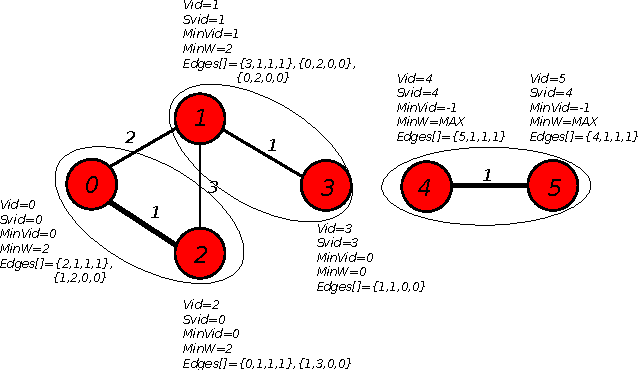
\includegraphics[width=0.5\textwidth]{img/pic.pdf}
\caption{Illustration of the Boruvka's algorithm: second iteration of the main loop, the minimal external edge search
	is completed.}
\label{evaluation:amd_stride}
\end{figure}

\section{Evaluation results}
\subsection {Platforms}
\subsection {Results}

%\begin{figure}[!tb]
%\centering
%\includegraphics[width=0.5\textwidth]{plots/{mst_boruvka_naive.rmat.s22.k4.plot}.pdf}
%\caption{Performance of Boruvka's algorithm (naive)}
%\label{evaluation:stream}
%\end{figure}

\begin{figure*}[!tb]
\centering
\includegraphics[width=0.9\textwidth]{img/timeline-rmat-s10-k16-ppn16-np16.png}
\caption{}
\label{evaluation:stream}
\end{figure*}

%\begin{thebibliography}{1}
%\end{thebibliography}

% that's all folks
\end{document}


